\documentclass[polish,a4paper,oneside,11pt]{article}
%\documentclass[polish,a4paper,twoside,11pt]{report}


%====PACKAGES
\usepackage[OT4]{fontenc}
\usepackage[utf8]{inputenc}
\usepackage[polish]{babel}
\usepackage{graphicx}
\usepackage{indentfirst}
\usepackage[a4paper,inner=3cm,outer=3cm,top=2.5cm,bottom=2.5cm,pdftex]{geometry}
\usepackage{listings}
\usepackage{color}
\usepackage{textcomp}
\usepackage{amsmath}
\usepackage{amsthm}
\usepackage{subfigure}
\usepackage{appendix}
\usepackage{multirow}
\usepackage{multicol}
\usepackage{longtable}
\usepackage{url}
\usepackage{array}
\usepackage{algorithm}

\floatname{algorithm}{Listing}

\linespread{1.3}

%//CAPTIONS FOR TABLE
\addto\captionspolish{%
  \renewcommand{\tablename}%
    {Tabela}%
}

\begin{document}

\thispagestyle{empty} %bez numeru strony

\begin{center}
{\large{Sprawozdanie z laboratorium:\\
Metaheurystyki i obliczenia inspirowane biologicznie}}

\vspace{3ex}

Zastosowanie algorytmów lokalnego przeszukiwania dla asymetrycznego problemu komiwojażera

\vspace{3ex}
{\footnotesize\today}

\end{center}


\vspace{10ex}

Prowadzący: dr inż. Maciej Komosiński

\vspace{5ex}

Autorzy:
\begin{tabular}{lllr}
\textbf{Mateusz Cicheński} & inf84780 & ISWD & hrkm@poczta.fm \\
\textbf{Artur Jaworski} & inf84813 & ISWD & Artur.A.Jaworski@gmail.com \\
\end{tabular}

\vspace{5ex}

Zajęcia poniedziałkowe, 13:30.


\newpage


\tableofcontents 
\cleardoublepage
\section{O problemie}
\subsection{Definicja problemu}
Problem komiwojażera można zdefiniować na wiele sposobów, w poniższym sprawozdaniu zostanie przytoczona definicja oparta o teorię grafów. W ogólności problem polega na znalezieniu optymalnej (tu - najkrótszej) trasy, która umożliwi odwiedzenie wszystkich docelowych miast dokładnie jeden raz. Problem ten jest problemem silnie NP trudnym.

Definicja brzmi następująco: Niech $G(V,A)$ oznacza dowolny graf skierowany, taki, że wierzchołki $V$ reprezentują zbiór wszystkich docelowych miast oraz istnieje łuk $A_{ij}$ z wierzchołka $i$ do wierzchołka $j$ jeśli istnieje połączenie z miasta $i$ do miasta $j$ i posiada on długość odpowiadającą odległości między tymi miastami. W tak zdefiniowanym grafie poszukujemy cyklu hamiltona o najmniejszej długości, który stanowi najkrótszą trasę umożliwiającą odwiedzenie wszystkich tras.

Z tej definicji mogą wyniknąć dwa problemy - brak połączenia między daną parą miast lub w ogólności brak cyklu hamiltona. Obydwa problemy można rozwiązać dodając na miejsce nieistniejących połączeń połączenia o bardzo dużej długości znacznie przewyższającej pozostałe długości łuków.

\subsection{Zastosowania i wariacje oryginalnego problemu}
Potencjalne zastosowania to próba zamodelowania i odnalezienia najszybszej trasy w mieście z uwzględnieniem czasów przejazdu daną ulicą jako długości łuków (wówczas ulice zakorkowane byłyby bardzo długie i można je próbować ominąć). Nawet uwzględniając tylko faktyczną długość ulicy można zastosować ten problem do znalezienia najlepszej trasy od punktu A do punktu B w aplikacji nawigującej. Oczywiście modyfikuje to nieco funkcję celu (nie doliczamy drogi powrotnej), ale jest to nadal ten sam problem.

Ponadto często rezygnuje się z kilku założeń problemu, np. zakazu odwiedzania dwukrotnie tego samego miasta czy przyjmuje się, że odległości między miastami spełniają nierówność trójkąta. Są to przypadki szczególne dla ogólnego sformułowania problemu komiwojażera i często okazuje się, że przy tych dodatkowych założeniach można zastosować heurystyki wykorzystające je w celu znajdowania lepszych rozwiązań w krótszym czasie. My jednak skupimy się na oryginalnym sformułowaniu i wszystkie doświadczenia przeprowadzane będą dla oryginalnego problemu.
\section{Rozwiązanie i operatory sąsiedztwa}
\subsection{Reprezentacja rozwiązania}
Dla porządku i nadania sensowności dalszym rozważaniom należy krótko wspomnieć czym jest rozwiązanie problemu i jaką formę reprezentacji tego rozwiązania przyjęliśmy. Rozwiązaniem, jak już zostało wspomniane w poprzednim punkcie, jest kolejność odwiedzanych miast. Wykorzystujemy przy tym założenie o tym, że dane miasto musi być odwiedzone dokładnie jeden raz, ponieważ mogłoby się zdarzyć, że z miasta A do B jest dalej niż gdyby jechać z miasta A do C a potem do B. Oczywiście w teorii taka sytuacja jest wyeliminowana przez minimalizację funkcji celu (jaką jest sumaryczna długość trasy), która automatycznie wybrałaby wówczas sytuację A-C-B. Korzystamy zatem z oryginalnej macierzy odległości, którą możnaby było poddać procesowi poszukiwania najkrótszej ścieżki między każdą parą miast, ale wówczas mogłoby wyjść na to, że dane miasto jest odwiedzone więcej niż jeden raz. Oczywiście takie stwierdzenie jest słuszne tylko w wypadku braku założeń odnośnie odległości między miastami (przykładowe założenie to spełnienie nierówności trójkąta między dowolnymi trójkami miast).

Stąd rozwiązanie to po prostu tablica jednowymiarowa o długości $n$ zawierająca na kolejnych pozycjach miasta, które powinny być odwiedzone w kolejności wynikającej z tej tablicy. Funkcję celu można szybko wyliczyć sumując odległości między kolejnymi parami miast występującymi w tabeli z uwzględnieniem połączenia między ostatnim i pierwszym miastem.

\subsection{Operator 2-OPT}

Wykorzystaliśmy najprostszy z operatorów sąsiedztwa, jakim jest 2-OPT. Jego zasada generowania sąsiadów jest bardzo prosta -- wybieramy dwa losowe punkty w rozwiązaniu i zamieniamy ze sobą miejscami. W ten sposób uzyskujemy nowe rozwiązanie (być może lepsze, być może gorsze). Bardzo łatwo można wykazać, że dla danego rozwiązania można wygenerować $\frac{n(n-1)}{2}$ sąsiadów. Wynika to z tego, że wpierw wybieramy 1 z $n$ pozycji rozwiązania, następnie 1 z $n-1$ pozostałych miejsc i je zamieniamy. Ponieważ przykładowo zamiana miejsca 3 z miejscem 8 da takiego samego sąsiada jak zamiana miejsca 8 z miejscem 3, to dzielimy uzyskaną liczbę przez 2.

\subsection{Operator 2-OPT dla TS i SA}

Dla algorytmów Tabu Search i Simulated Annealing przygotowaliśmy osobny operator 2-OPT, który umożliwia generowanie sąsiedztwa zgodnie z zasadą oryginalnego operatora poprzez zamianę miejscami dwóch pozycji w rozwiązaniu. Różnica polega na tym, że zamiany nie są deterministyczne -- pozycje są wybierane losowo. Dzięki temu zabiegowi wygenerowanie każdego sąsiada jest równie prawdopodobne; unikamy więc ukierunkowania w jedną ,,stronę'' generowanych sąsiadów.
\section{Porównanie działania algorytmów}
Testy algorytmów zostały przeprowadzone na grupie 10 instancji testowych o różnym rozmiarze: od 33 do 403 miast. Na każdej z instancji każdy z algorytmów został uruchomiony dziesięciokrotnie w celu ustalenia zarówno wartości średniej jak i rozproszenia poszczególnych mierzonych parametrów. Testy przeprowadzono na maszynie wyposażonej w procesor Intel Core i7-620M oraz 4GB pamięci RAM. 

Zaimplementowane algorytmy to algorytm losowy, dwa algorytmy przeszukiwania lokalnego -- greedy oraz steepest, a także prosta heurystyka. W jej formie użyto algorytmu zachłannego, który po wylosowaniu punktu startowego przechodzi do najbliższego z sąsiadów, który nie został jeszcze odwiedzony.

Wyniki zostaną obecnie zaprezentowane w poszczególnych punktach.

\subsection{Jakość działania}
Optymalne wartości funkcji celu dla każdej instancji były znane a priori, dlatego też jako miarę jakości działania algorytmów wykorzystano następującą zależność:
\begin{equation*}
fitness = \frac{f_{alg}(\Pi_i)}{f_{OPT}(\Pi_i)}*100\%
\end{equation*}
gdzie:

\begin{table}[h!]
       \begin{tabular}{lll}
       	$fitness$ & - & jakość algorytmu\\ 
        $f_{alg}(\Pi_{i})$ & - & wartość funkcji celu rozwiązania zwracanego przez badany \\
        &&algorytm dla instancji $\Pi_i$\\ 
		$f_{OPT}(\Pi_{i})$ & - & wartość funkcji celu rozwiązania optymalnego dla instancji $\Pi_i$
		\end{tabular}
\end{table}
\noindent Jeżeli algorytm zwróci rozwiązanie optymalne, miara jakości wyniesie 100\%. Wraz z pogarszaniem się zwracanego wyniku miara jakości będzie rosła, wyznaczając stosunkowy stopień oddalenia od wartości optymalnej.

\begin{figure}[!h]
\centering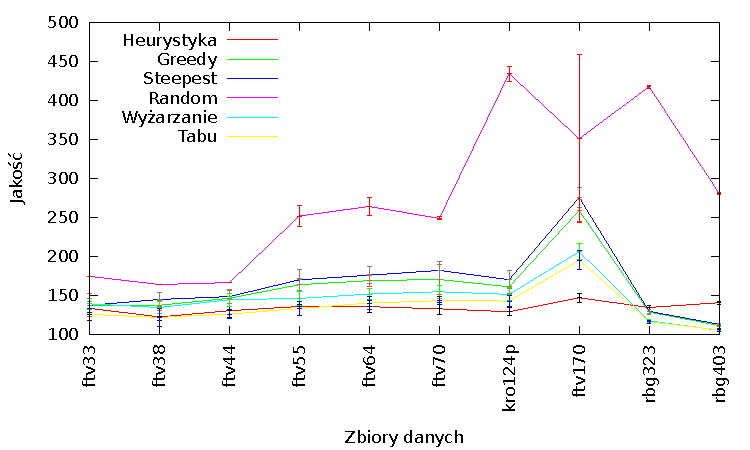
\includegraphics[width=12cm]{img/jakosc_avg}
\caption{Jakość działania poszczególnych algorytmów dla przypadku średniego. Na niebiesko czas działania heurystyki, na czerwono algorytmu Greedy, na zielono algorytmu Steepest, a na fioletowo czas działania algorytmu losowego.}\label{rys:jakosc_avg}
\end{figure}

\begin{figure}[!h]
\centering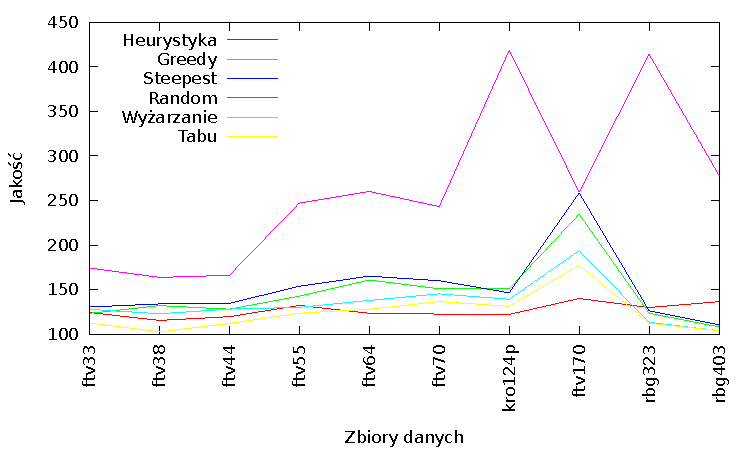
\includegraphics[width=12cm]{img/jakosc_best}
\caption{Jakość działania poszczególnych algorytmów dla przypadku najlepszego. Na niebiesko czas działania heurystyki, na czerwono algorytmu Greedy, na zielono algorytmu Steepest, a na fioletowo czas działania algorytmu losowego.}\label{rys:jakosc_best}
\end{figure}

Rysunki \ref{rys:jakosc_avg} oraz \ref{rys:jakosc_best} przedstawiają wyniki testów jakości odpowiednio dla przypadku średniego i najlepszego. Najlepsze wyniki zostają zwracane przez heurystykę. Jakość działania algorytmów przeszukiwania lokalnego jest bardzo zbliżona. Najgorzej wypada algorytm losowy -- przy mniejszych instancjach zwracane przez niego wyniki nie odbiegają jeszcze tak bardzo jakościowo od pozostałych algorytmów, wraz z liniowym wzrostem rozmiaru instancji rozmiar przestrzeni rozwiązań dopuszczalnych rośnie jednak wykładniczo, przez co proste strzelanie w wynik staje się probabilistycznie dużo mniej opłacalne.

Jeżeli chodzi o rozproszenie jakości zwracanych rozwiązań, wyniki zwracane przez heurystykę są bardzo zbliżone. Algorytmy lokalny zwracają wyniki nieznacznie bardziej rozrzucone wokół wartości średniej. Algorytm losowy zachowuje się natomiast całkowicie losowo -- widzimy tu przypadki od praktycznie zerowego rozrzucenia, przez to porównywalne do algorytmów lokalnych, kończąc na kilkukrotnie od nich wyższym.

Porównując wykresy dla przypadku średniego i najlepszego zauważyć można wyraźnie, że tendencja jest zachowana, jedynie wykresy znajdują się o kilka punktów procentowych niżej.

\subsection{Czas}
Do pomiaru czasu skorzystano z timera udostępnionego razem z biblioteką \emph{boost}. Zwraca on wynik w postaci wartości podwójnej precyzji (\texttt{double}), rozpoczynając od $0,001$s. W celu dokładniejszego wyznaczenia czasu wywołań algorytmów dla najmniejszych instancji, powtarzano uruchamianie z tego samego punktu startowego minimalnie przez $0,5$s, po czym otrzymany czas dzielono przez liczbę wykonań algorytmu.

\begin{figure}[!h]
\centering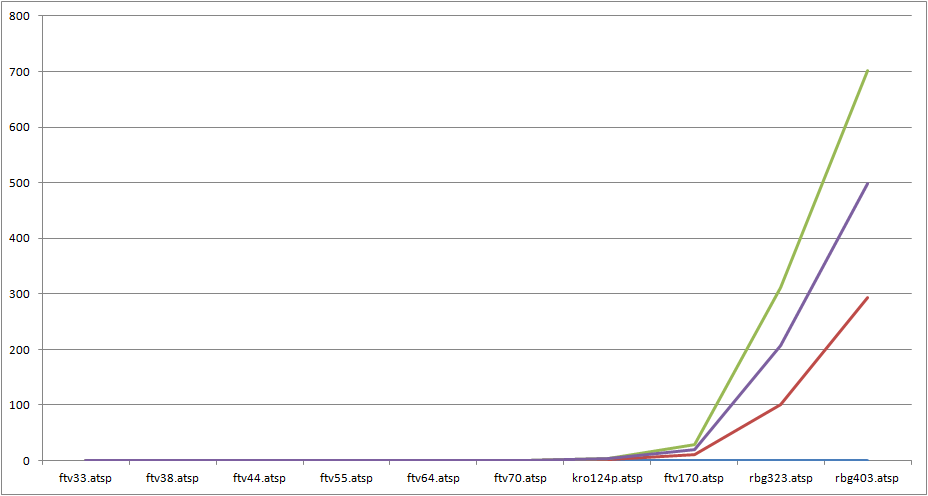
\includegraphics[width=12cm]{img/czas_avg}
\caption{Czas działania poszczególnych algorytmów dla przypadku średniego. Na niebiesko czas działania heurystyki, na czerwono algorytmu Greedy, na zielono algorytmu Steepest, a na fioletowo czas działania algorytmu losowego.}\label{rys:czas_avg}
\end{figure}

Rysunek \ref{rys:czas_avg} przedstawia wyniki badania czasu działania poszczególnych algorytmów dla przypadku średniego. Ponownie, najlepiej spisała się heurytyka, która posiada złożoność $O(n^2)$, co nawet dla największej badanej instancji daje wynik nieprzekraczający $0,01$s. Na drugim miejscu znalazł się algorytm greedy, który szybciej niż algorytm steepest odwiedza kolejnych sąsiadów. Ten drugi algorytm spisał się najgorzej, gdyż przed przejściem do kolejnego sąsiada musi przejrzeć wszystkich swoich sąsiadów ($\frac{n(n-1)}{2}$).

Algorytm losowy nie kończy się w sposób naturalny. W celu zachowania równych szans, timeout dla tego algorytmu został określony na poziomie średniej arytmetycznej czasu działania algorytmów greedy i steepest. Jako, że czas działania został ustalony w sposób sztuczny, analizowanie go byłoby bezpodstawne.

\subsection{Współczynnik czas/jakość}
Wybierając algorytm nie zawsze interesuje nas to, by algorytm zwracał za wszelką cenę rozwiązanie jak najbardziej zbliżone do optymalnego. Czasami jesteśmy skłonni poświęcić odrobinę jakości kosztem krótszego czasu działania, szczególnie w systemach czasu rzeczywistego. Dlatego też konieczne jest wyznaczenie wartości, która uwzględniałaby oba te czynniki naraz.

Jako pierwszy krok, z wyników przeprowadzonych testów (również na innych instancjach niż te omawiane w poniższym sprawozdaniu) wybrano najlepsze i najgorsze wartości dla czasu i jakości. Wyniosły one odpowiednio $0,001$s i $754,89$s oraz $100\%$ i $542,76\%$. Następnie, średnie wyniki czasu działania i jakości badanych algorytmów znormalizowano do wartości z przedziału $<0,1>$ - $0$ dla rozwiązania najgorszego, $1$ dla najlepszego. Korzystając z tych znormalizowanych wartości przystąpiono do wyznaczenia współczynnika cena/jakość zgodnie ze wzorem na ważoną średnią harmoniczną:
\begin{equation*}
price\_fitness = \frac{2}{\frac{1}{time_{norm} + \epsilon} + \frac{1}{fitness_{norm} + \epsilon} }
\end{equation*}

Do wartości znormalizowanych współczynników czasu i jakości dodajemy nieskończenie małą wartość $\epsilon$ w celu uniknięcia dzielenia przez 0. Wówczas jeśli którykolwiek z tych współczynników wyniesie $0$ dla danego algorytmu, to we wzorze na współczynnik ceny do jakości uzyskamy $\frac{2}{\frac{1}{time_{norm} + \epsilon} + \frac{1}{0 + \epsilon}}$, co oznacza, że mamy $\frac{2}{1 + \infty}$, czyli ostatecznie $0$.

Algorytm działający w najkrótszym czasie, zwracający najlepszy wynik, otrzyma współczynnik cena/jakość równy $1$, najgorszy - $0$. Słaba wartość któregokolwiek ze znormalizowanych czynników natychmiast obniża wartość współczynnika. Jednak przykładowo algorytm zwracający najlepsze rozwiązania, ale działający najwolniej otrzyma wartość współczynnika równą 0.

\begin{figure}[!h]
\centering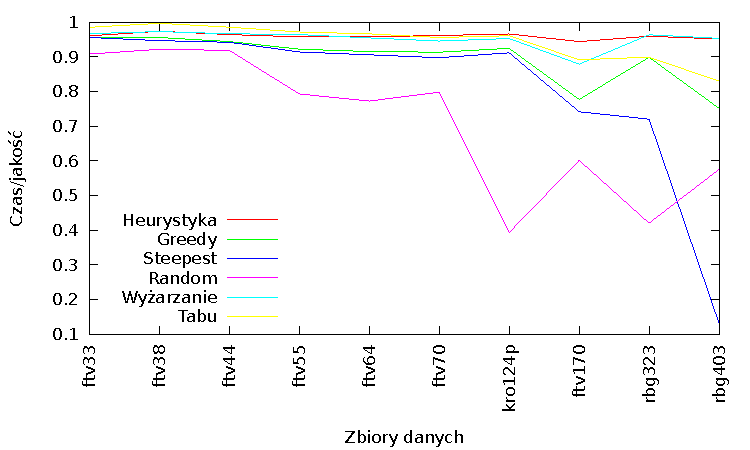
\includegraphics[width=12cm]{img/jakosc-czas}
\caption{Współczynnik czas/jakość dla poszczególnych instancji i poszczególnych algorytmów dla przypadku średniego. Na niebiesko czas działania heurystyki, na czerwono algorytmu Greedy, na zielono algorytmu Steepest, a na fioletowo czas działania algorytmu losowego.}\label{rys:czas_jakosc}
\end{figure}

Jako, że heurystyka spisała się najlepiej zarówno pod względem czasu jak i jakości zwracanych wyników, jej współczynnik czas/jakość niemalże sięga wartości $1$. Na drugim miejscu znalazł się algorytm greedy, który wygrał z algorytmem steepest głównie na gruncie czasu działania. Algorytm random po raz kolejny zachowuje się nieprzewidywalnie, wraz ze wzrostem instancji wartość jego współczynnika czas/jakość spada, głównie za sprawą zdecydowanego spadku w jakości zwracanych rozwiązań.

\subsection{Średnia liczba kroków oraz ocenionych rozwiązań algorytmów przeszukiwania lokalnego}
Algorytmy steepest i greedy działają w odmienny sposób. Steepest, zanim przejdzie do któregoś z sąsiadów, przegląda wszystkich swoich sąsiadów w celu znalezienia tego najlepszego. Greedy natomiast po trafieniu na pierwszego lepszego od siebie sąsiada natychmiast do niego przechodzi. Oznacza to, że steepest powinien docierać do wyniku w mniejszej liczbie kroków (każdy krok wiąże się z probabilistycznie wyższą różnicą funkcji celu), jednak przeglądając większą liczbę rozwiązań.

\begin{figure}[!h]
\centering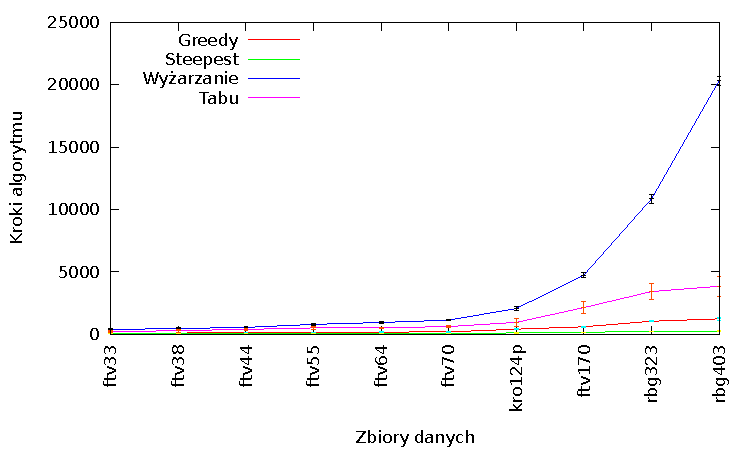
\includegraphics[width=12cm]{img/loc_skoki}
\caption{Średnia liczba kroków w dojściu do optimum lokalnego. Na czerwono wartości dla algorytmu Steepest, na niebiesko wartości dla algorytmu Greedy.}\label{rys:loc_skoki}
\end{figure}

\begin{figure}[!h]
\centering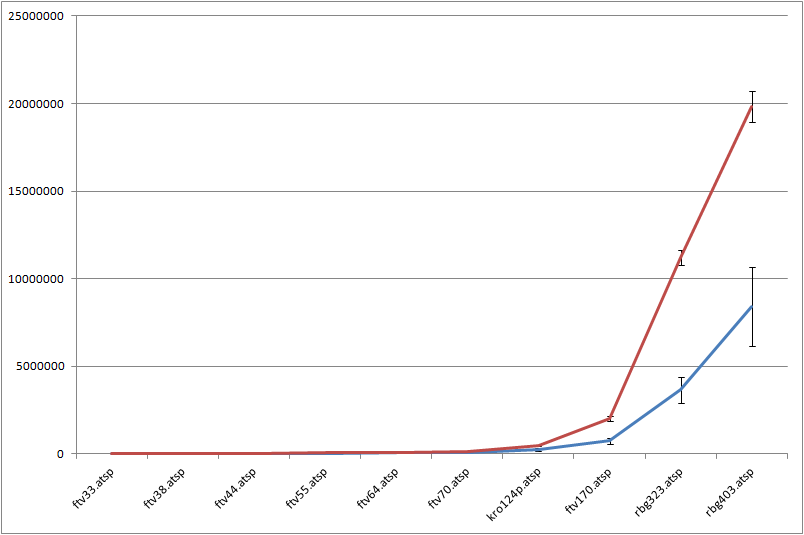
\includegraphics[width=12cm]{img/loc_sasiedzi}
\caption{Średnia liczba przejrzanych rozwiązań w dojściu do optimum lokalnego. Na czerwono wartości dla algorytmu Steepest, na niebiesko wartości dla algorytmu Greedy.}\label{rys:loc_sasiedzi}
\end{figure}

Rysunki \ref{rys:loc_skoki} i \ref{rys:loc_sasiedzi} dokładnie wpisują się w przedstawione wcześniej hipotezy. Algorytm greedy faktycznie dochodzi do lokalnego optimum wykonując więcej mniejszych skoków, natomiast algorytm steepest przegląda większą liczbę rozwiązań sąsiednich.
\section{Poprawa jakości rozwiązania w algorytmach LS na przykładzie algorytmów Greedy oraz Steepest}
\subsection{Instancja br17.atsp}
\begin{figure}[!h]
\centering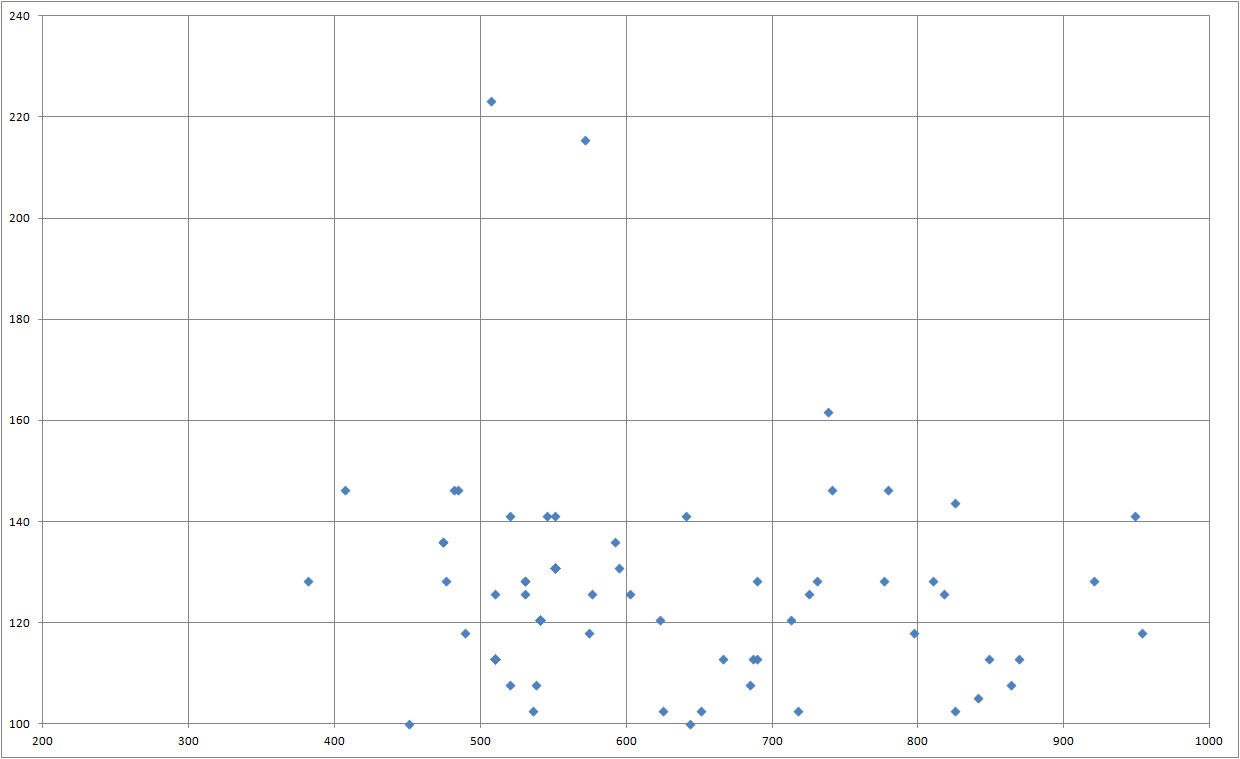
\includegraphics[width=12cm]{img/br17_b2e_g.png}
\caption{Poprawa jakości algorytmu Greedy dla instancji br17. Na osi pionowej odłożono procentowe wartości rozwiązania końcowego, na osi poziomej z kolei procentowe wartości rozwiązania startowego względem znanego optimum. Punkty przedstawiają poszczególne rozwiązania uzyskane przez kolejne uruchomienia algorytmu dla tej samej instacji, lecz dla innych punktów startowych.}\label{rys:br17g}
\end{figure}
\begin{figure}[!h]
\centering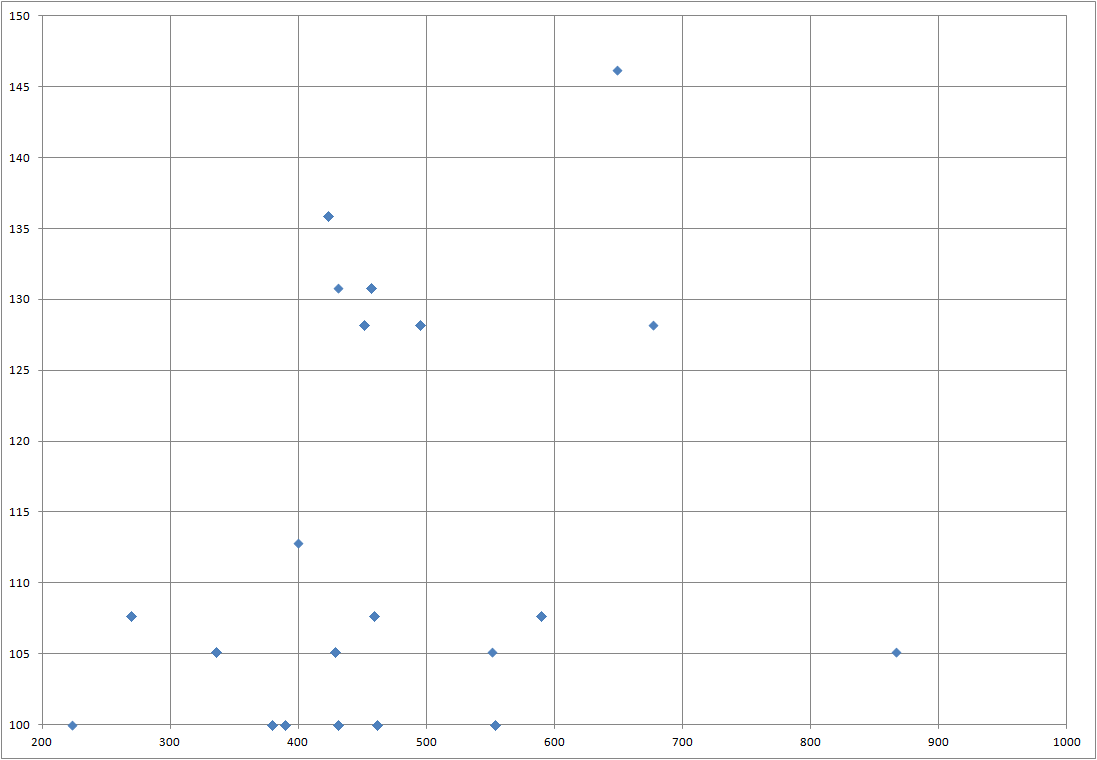
\includegraphics[width=12cm]{img/br17_b2e_s.png}
\caption{Poprawa jakości algorytmu Steepest dla instancji br17. Na osi pionowej odłożono procentowe wartości rozwiązania końcowego, na osi poziomej z kolei procentowe wartości rozwiązania startowego względem znanego optimum. Punkty przedstawiają poszczególne rozwiązania uzyskane przez kolejne uruchomienia algorytmu dla tej samej instacji, lecz dla innych punktów startowych.}\label{rys:br17s}
\end{figure}

Dla tej instacji obydwa algorytmy zachowywały się dość ciekawie co zaprezentowano na rysunku \ref{rys:br17g} i \ref{rys:br17s}. Okazuje się, że Steepest znalazł kilkukrotnie rozwiązanie optymalne i zasadniczo znajdował lepsze rozwiązania niż Greedy. Można zauważyć, że taktyka przeskakiwania od razu do lepszego rozwiązania, a nie przeglądanie wszystkich sąsiadów dookoła jest dla tej instancji całkiem dobra, ponieważ prawie zawsze znajdowano rozwiązanie o conajwyżej 50\% gorsze od optimum. Dwa przypadki, kiedy algorytm Greedy nie zadziałał tak skutecznie świadczą o tym, że musiało istnieć pewne lokalne minimum, w które właśnie ten algorytm ma większą szansę wpaść aniżeli Steepest, ponieważ nie przegląda całego sąsiedztwa aktualnie analizowanego rozwiązania. Ma więc tendencje do zeskakiwania w złym kierunku (ku gorszemu minimum lokalnemu).

\subsection{Instancja ftv33.atsp}
\begin{figure}[!h]
\centering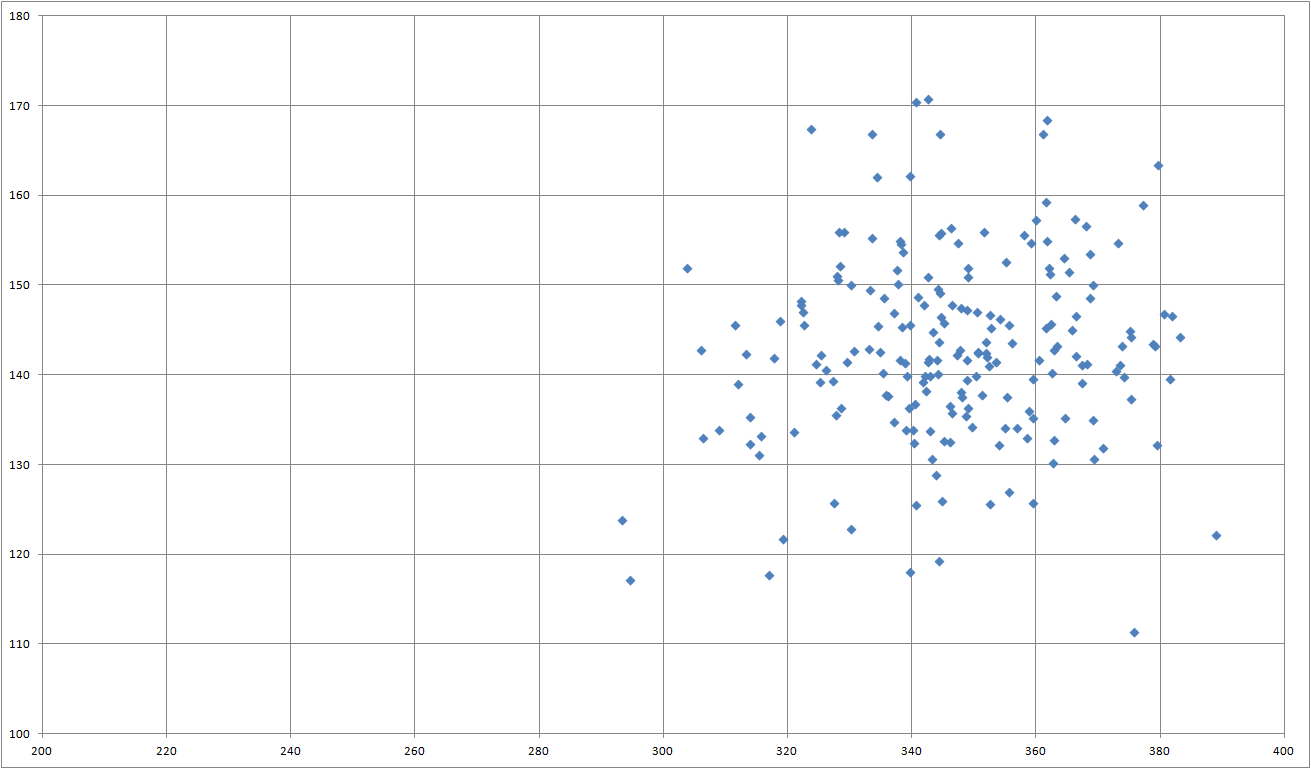
\includegraphics[width=12cm]{img/ftv33_b2e_g.png}
\caption{Poprawa jakości algorytmu Greedy dla instancji ftv33. Na osi pionowej odłożono procentowe wartości rozwiązania końcowego, na osi poziomej z kolei procentowe wartości rozwiązania startowego względem znanego optimum. Punkty przedstawiają poszczególne rozwiązania uzyskane przez kolejne uruchomienia algorytmu dla tej samej instacji, lecz dla innych punktów startowych.}\label{rys:ftv33g}
\end{figure}
\begin{figure}[!h]
\centering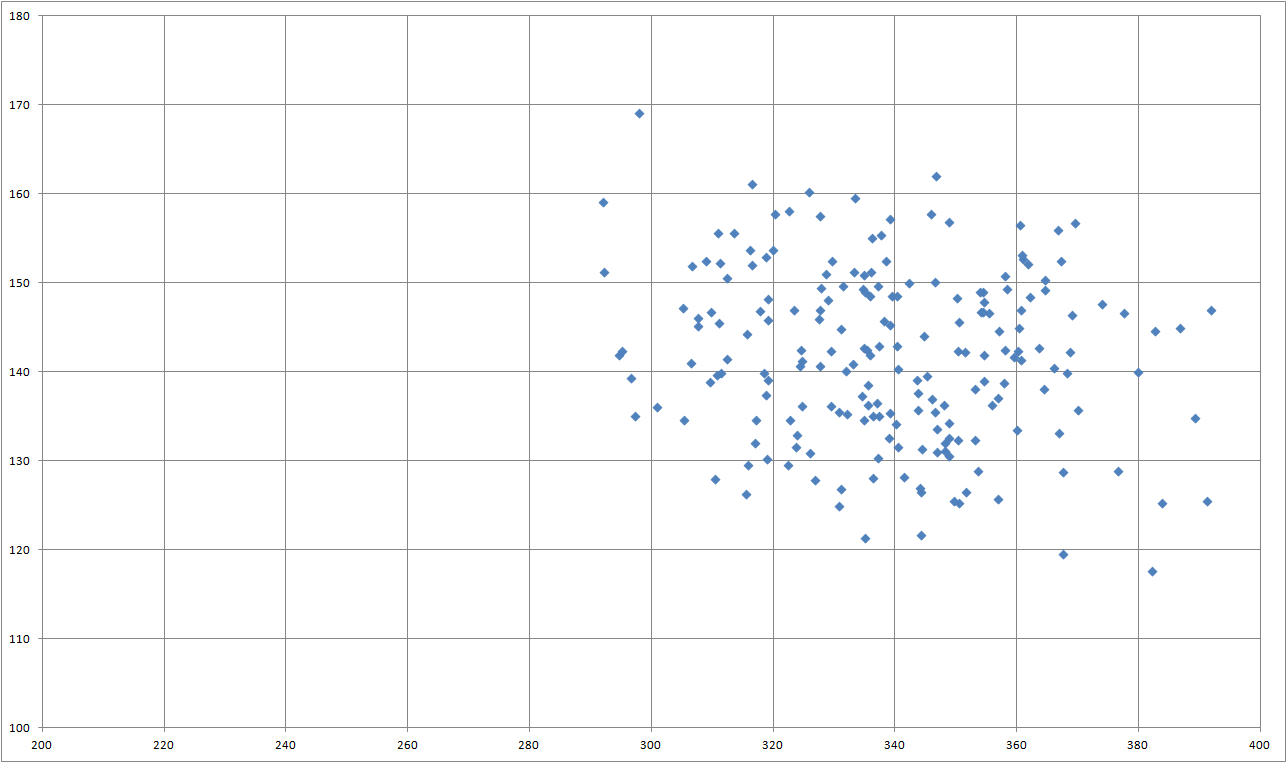
\includegraphics[width=12cm]{img/ftv33_b2e_s.png}
\caption{Poprawa jakości algorytmu Steepest dla instancji ftv33. Na osi pionowej odłożono procentowe wartości rozwiązania końcowego, na osi poziomej z kolei procentowe wartości rozwiązania startowego względem znanego optimum. Punkty przedstawiają poszczególne rozwiązania uzyskane przez kolejne uruchomienia algorytmu dla tej samej instacji, lecz dla innych punktów startowych.}\label{rys:ftv33s}
\end{figure}

Ta instancja pokazuje przewagę dokładniejszego przeszukiwania sąsiedztwa przez algorytm Steepest nad pochopnym skakaniem do pierwszego znalezionego rozwiązania, które jest lepsze. Na rysunku \ref{rys:ftv33g} i \ref{rys:ftv33s} widać, że tendencja obydwu algorytmów jest bardzo podobna i odnajdują głównie rozwiązania odległe od optimum od 20\% do 50\%. Jednak co ciekawe algorytm Greedy kilkukrotnie trafił na lepsze rozwiązania niż Steepest. A więc nie wpadł w pierwszy lepszy ,,dołek'', tylko go ominął i trafił na lepszy zbiór rozwiązań.

\subsection{Wnioski dotyczące jakości rozwiązania względem liczby uruchomień algorytmu}
Powyższe dwa przykłady pokazują, że obydwa podejścia różnią się tolerancją na kształt krajobrazu rozwiązań. Algorytm Greedy ma większą łatwość w przeskakiwaniu lokalnych minimów, dzięki czemu może trafić na lepsze rozwiązania jeśli balansuje na krawędzi dwóch lokalnych minimów. Oczywiście jego skuteczność zależy od kolejności przeglądania sąsiadów i kształtu krajobrazu. Z kolei algorytm Steepest zawsze ,,leci'' w ustalonym kierunku. Od początku obiera pewne minimum lokalne za swój cel i zasadniczo można powiedzieć, że jest w związku z tym bardziej deterministyczny (co szczególnie widać na rysunku \ref{rys:br17s}, gdzie większość punktów się bardzo pokrywa, stąd jest ich tam wizualnie mniej). Można też zauważyć, że uzyskana poprawa jakości rozwiązania dla danej instancji bez względu na wykorzystany algorytm okazuje się oscylować wokół podobnych wartości.
\section{Czy opłaca się powtarzać uruchamianie algorytmów LS?}
\section{Ocena podobieństwa znajdowanych rozwiązań lokalnie optymalnych dla wybranych instancji}
W celu porównania podobieństwa rozwiązań zwracanych przez algorytmy optymalizacji lokalnej zaproponowano następującą miarę podobieństwa. Kolejne miasta w jednym z rozwiązań są po kolei sprawdzane z drugim rozwiązaniem. Jeżeli w jednym i drugim rozwiązaniu miasto następująco po aktualnie sprawdzanym mieście (uwzględniając połączenie miasta ostatniego z miastem pierwszym w rozwiązaniu) jest takie samo, inkrementowany jest licznik podobieństw. Na koniec, licznik podobieństw jest dzielony przez długość rozwiązania, przez otrzymujemy znormalizowaną wartość z zakresu $<0-1>$.

Przedstawmy obecnie działanie zaproponowanej miary na przykładzie. Dane są dwie instancje - $3-1-2-4-0$ oraz $2-4-1-0-3$. Kolejne kroki algorytmu przedstawione są w poniższej tabeli.

\begin{tabular}{|l|l|l|}
		\hline
		Rozwiązanie 1 & Rozwiązanie 2 & Licznik podobieństw\\
		\hline
		& & 0 \\
		3-1 & 3-2 & 0 \\
		1-2 & 1-0 & 0 \\
		2-4 & 2-4 & 1 \\
		4-0 & 4-1 & 1 \\
		0-3 & 0-3 & 2\\
		\hline
\end{tabular}

\noindent Uzyskany licznik podobieństw należy jeszcze podzielić przez długość rozwiązania ($5$), przez co otrzymujemy współczynnik podobieństwa instancji wynoszący $0,4$.

Obecnie przedstawione zostaną wyniki porównania rozwiązań zwracanych dla algorytmu steepest i greedy. Przeprowadzono testy polegające na 10-krotnym uruchomieniu algorytmów z tego samego losowego punktu startowego dla dwóch instancji: flv33.atsp oraz ftv55.atsp. Następnie obliczono miary podobieństwa wyników zwróconych przez tak uruchomione algorytmy. Wyniki przedstawione zostały w tabelach \ref{tab:sim_33} i \ref{tab:sim_55}. W kolumnach ustawione są kolejne uruchomienia algorytmu steepest, natomiast w wierszach algorytmu greedy. Elementy na głównej przekątnej informują o tym jak podobne rozwiązania zwracają algorytmy gdy startują z tego samego punktu, czy trafiają w to samo optimum lokalne, natomiast wartości poza główną przekątną mogą mówić więcej o istnieniu małej liczby lub nawet tylko jednego optimum lokalnego - mimo startu z różnych miejsc algorytmy ''staczają się'' w to samo miejsce.

\begin{table}[h!]
	\centering
       \begin{tabular}{|l|l|l|l|l|l|l|l|l|l|l|}
        \hline
		& 1 & 2 & 3 & 4 & 5 & 6 & 7 & 8 & 9 & 10 \\
		\hline
		1 & \textbf{0.29} & 0.35 & 0.29 & 0.26 & 0.24 & 0.21 & 0.21 & 0.29 & 0.35 & 0.32 \\    
		2 & 0.44 & \textbf{0.38} & 0.32 & 0.18 & 0.41 & 0.18 & 0.12 & 0.35 & 0.44 & 0.35 \\    
		3 & 0.32 & 0.21 & \textbf{0.24} & 0.47 & 0.29 & 0.24 & 0.26 & 0.18 & 0.24 & 0.32 \\ 
		4 &	0.29 & 0.26 & 0.29 & \textbf{0.15} & 0.29 & 0.26 & 0.32 & 0.24 & 0.15 & 0.29 \\   
		5 & 0.26 & 0.12 & 0.15 & 0.12 & \textbf{0.18} & 0.29 & 0.26 & 0.15 & 0.21 & 0.21 \\   
		6 & 0.26 & 0.35 & 0.18 & 0.18 & 0.26 & \textbf{0.32} & 0.21 & 0.29 & 0.29 & 0.26 \\   
		7 & 0.29 & 0.47 & 0.38 & 0.32 & 0.38 & 0.12 & \textbf{0.24} & 0.44 & 0.35 & 0.41 \\   
		8 & 0.32 & 0.12 & 0.18 & 0.24 & 0.24 & 0.29 & 0.41 & \textbf{0.18} & 0.18 & 0.29 \\   
		9 & 0.09 & 0.21 & 0.24 & 0.15 & 0.29 & 0.24 & 0.21 & 0.21 & \textbf{0.26} & 0.21 \\   
		10 & 0.35 & 0.12 & 0.26 & 0.29 & 0.24 & 0.18 & 0.21 & 0.32 & 0.18 & \textbf{0.24} \\
		\hline
		\end{tabular}
		\caption{Podobieństwo zwracanych rozwiązań dla instancji ftv33.atsp. W kolumnach algorytm steepest, w wierszach algorytm greedy, wytłuszczone elementy to podobieństwo wyników zwracanych dla tego samego punktu startowego.}
		\label{tab:sim_33}
\end{table}

\begin{table}[h!]
       \centering
       \begin{tabular}{|l|l|l|l|l|l|l|l|l|l|l|}
        \hline
		& 1 & 2 & 3 & 4 & 5 & 6 & 7 & 8 & 9 & 10 \\
		\hline
		1 & \textbf{0.14} & 0.21 & 0.21 & 0.2 & 0.2 & 0.16 & 0.29 & 0.21 & 0.14 & 0.18 \\
		2 & 0.32 & \textbf{0.29} & 0.13 & 0.23 & 0.21 & 0.2 & 0.25 & 0.2 & 0.38 & 0.13 \\   
		3 & 0.32 & 0.16 & \textbf{0.25} & 0.16 & 0.13 & 0.18 & 0.29 & 0.32 & 0.16 & 0.25 \\   
		4 & 0.36 & 0.18 & 0.2 & \textbf{0.27} & 0.21 & 0.21 & 0.23 & 0.21 & 0.27 & 0.16 \\   
		5 & 0.41 & 0.23 & 0.25 & 0.25 & \textbf{0.36} & 0.16 & 0.36 & 0.2 & 0.23 & 0.16 \\   
		6 & 0.27 & 0.29 & 0.2 & 0.18 & 0.29 & \textbf{0.23} & 0.34 & 0.21 & 0.2 & 0.16 \\   
		7 & 0.29 & 0.23 & 0.13 & 0.3 & 0.2 & 0.2 & \textbf{0.29} & 0.25 & 0.14 & 0.29 \\   
		8 & 0.21 & 0.18 & 0.2 & 0.21 & 0.21 & 0.21 & 0.23 & \textbf{0.32} & 0.2 & 0.21 \\   
		9 & 0.34 & 0.25 & 0.23 & 0.25 & 0.2 & 0.21 & 0.27 & 0.2 & \textbf{0.29} & 0.25 \\   
		10 & 0.29 & 0.2 & 0.18 & 0.29 & 0.2 & 0.29 & 0.29 & 0.16 & 0.25 & \textbf{0.21} \\
		\hline
		\end{tabular}
		\caption{Podobieństwo zwracanych rozwiązań dla instancji ftv55.atsp. W kolumnach algorytm steepest, w wierszach algorytm greedy, wytłuszczone elementy to podobieństwo wyników zwracanych dla tego samego punktu startowego.}
		\label{tab:sim_55}
\end{table}

Analizując przedstawione tabele możemy dojść do wniosku, że obydwie instancje są zróżnicowane w równomierny sposób. Nawet startując z tych samych punktów algorytmy trafiają na optima lokalne w niewielkim stopniu do siebie podobne. Globalnie również musi istnieć wiele lokalnych ektremów, gdyż elementy poza główną przekątną nie osiągają wysokich wartości podobieństwa.
\section{Wnioski}
Zbierzmy obecnie komentarze występujące w ninejszej pracy w całość. Do rozwiązania problemu ATSP najlepszym algorytmem okazała się zachłanna heurystyka. Działa ona najszybciej i zwraca najlepsze wyniki. Algorytmy przeszukiwania lokalnego pod względem jakości nie odbiegają w znaczącym stopniu od heurystyki, jednak dużo dłużej szukają lokalnego optimum. W ogólności jednak heurystyka startująca z danego punktu, działająca w sposób deterministyczny (przeglądając sąsiadów zawsze w tej samej kolejności) może rozwiązania optymalnego nigdy nie znaleźć, natomiast algorytm przeszukiwania lokalnego zawsze może wystartować z punktu leżącego na zboczu, które zaprowadzi go do ekstremum globalnego.

Porównując algorytmy steepest i greedy zauważamy, że mimo minimalnej tylko różnicy w kodzie, sprowadzającej się w gruncie rzeczy do dodania jednej instrukcji \texttt{break} w pętli, natura ich działania jest skrajnie różna. Algorytm greedy dużo szybciej zmienia sąsiadów, natomiast algorytm steepest przegląda ich dużo większą liczbę.
\section{Napotkane trudności}
Wymagania dotyczące sprawozdania można podzielić na kilka części. Są to: implementacja algorytmów pod wybrany problem, przygotowanie w odpowiedni sposób danych wyjściowych z działania algorytmów (w celu ułatwienia późniejszej obróbki danych), przygotowanie skryptu generującego wykresy oraz napisanie sprawozdania.

Punkt dotyczący implementacji wykonaliśmy dość szybko (na dwa tygodnie przed faktycznym terminem oddania sprawozdania), a wyniki zapisywane z kolejnych uruchomień posiadały już łatwe w obróbce formatowanie, także ten element nie sprawił nam większych trudności.

Niestety kwestia skryptu do wykresów jest ''w trakcie'', ponieważ nie zdążyliśmy go po prostu spreparować, a okazało się, że już zbliżył się termin oddania sprawozdania. W związku z tym wybraliśmy na chwilę obecną metodę ''szybką'', ale mało efektywną na dłuższą metę, czyli wygenerowanie potrzebnych wykresów przy pomocy Excel'a. Można oczywiście narzekać na to, że są one w postaci bitmapowej, jednak do wyciągania wniosków wydają się być wystarczające. Postaramy się, żeby w następnej wersji raportu wykresy były już porządnie splotowane.

Punkt dotyczący napisania sprawozdania został wypełniony, być może gdyby było więcej czasu, to uwzględnilibyśmy więcej elementów z sekcji ''nieobowiązkowe'', mimo wszystko wydaje nam się, że sprawozdanie zostało przygotowane w sposób rzetelny.
\section{Propozycje udoskonaleń i spodziewane efekty}
Przedstawione algorytmy można przede wszystkim bardzo łatwo i skutecznie zrównoleglić na wiele wątków, co zdecydowanie wpłynie na czas obliczeń -- więcej rozwiązań można przejrzeć w tym samym czasie, co daje probabilistycznie większe prawdopodobieństwo znalezienia optimum lub wartości zbliżonej do optimum aniżeli wersja jednowątkowa. Oczywiście uzyskany efekt jest zależny w tym wypadku od architektury komputera i nic nie da w przypadku jednoprocesorowego stanowiska obliczeniowego, ale w dzisiejszych czasach nie powinno to stanowić większego problemu.

Można by pokusić się o napisanie prostych funkcji uaktualniających wartość funkcji rozwiązania bez konieczność przeglądania całego rozwiązania, co na pewno umożliwiałoby zyskanie kilku cykli procesora na przeglądnięcie większej liczby rozwiązań. Jednak wydaje się, że uzyskany zysk czasowy nie wpłynąłby znacząco na ostateczne wyniki poszczególnych algorytmów (dotyczyłby algorytmu random, Greedy oraz Steepest w równym stopniu, więc końcowe wyniki byłyby tylko odpowiednio przeskalowane).

Wybór języka programowania \emph{C++} był podyktowany m.in. szybkością działania kompilowanego kodu (brak kodu pośredniego, który jest wykonywany przez wirtualną maszynę, tylko kod natywny pod dany system operacyjny), jednak ponownie wydaje się, że ta kwestia ma równorzędny wpływ na uzyskane wyniki każdego z algorytmów.

Na koniec istotne wydaje się odpowiednie dobieranie punktu startowego dla algorytmów lokalnego przeszukiwania zgodnie z zasadą ,,dobre rozwiązania powinny znajdować się stosunkowo blisko lepszych rozwiązań'', czyli odpalenie na początek heurystyki znajdującej właśnie dobre rozwiązanie, które będzie stanowiło podstawę do działania dla algorytmów przeszukiwania. Wówczas istnieje szansa, że trafimy na lepsze rozwiązanie z większym prawdopodobieństwem aniżeli startowanie z losowych rozwiązań (być może słabych jeśli chodzi o wartość). Wniosek ten jest prawdziwy, co można zaobserwować w Tabeli \ref{tab:heur_local}. Dla porównania, algorytmy Steepest i Greedy uruchamiane 10-krotnie z losowych punktów startowych uzyskały dla badanej instancji flv55.atsp wyniki odpowiednio 153,7 i 142,6. Uwzględniono w niej wybraną przez nas zachłanną heurystykę, która zgodnie z naszym doświadczeniem okazała się być lepsza niż algorytmy lokalnego przeszukiwania startujące z losowych punktów.

Przytoczona tabela pokazuje, że nie były to najlepsze wyniki, ponieważ udało się je poprawić przeglądając sąsiedztwa rozwiązań wskazanych przez heurystykę. Stąd płynie dość istotny wniosek, że korzystnie jest, gdy rozwiązanie początkowe, od którego startują algorytmy lokalnego przeszukiwania, jest wybrane w sposób nieprzypadkowy przy pomocy heurystyki, która już posiada dość dobre przybliżenie względem optimum. Oczywiście pojawia się tutaj problem dobrania odpowiedniej heurystyki do problemu i porównania różnych heurystyk między sobą. Jednak można przykładowo rozwiązać go ,,automatycznie'' wykorzystując algorytm ewolucyjny (genetyczny), gdzie do populacji początkowej trafiają rozwiązania wygenerowane przez różne heurystyki.

\begin{table}[h!]
	\centering
       \begin{tabular}{|l|l|l|}
        \hline
		Heurystyka & Heurystyka + Steepest & Heurystyka + Greedy \\
		\hline
		139.74 & 126.12 & 126.12 \\
		143.97 & 124.38 & 124.38 \\
		132.52 & 128.61 & 130.16 \\
		125.81 & 118.84 & 118.84 \\
		137.38 & 126 & 127.55 \\
		139.12 & 123.82 & 130.53 \\
		143.97 & 124.38 & 124.38 \\
		139.74 & 126.12 & 126.12 \\
		132.52 & 128.61 & 130.16 \\
		139.18 & 137.69 & 137.69 \\
		\hline
		\end{tabular}
		\caption{Jakość uzyskiwanych rozwiązań przy wykorzystaniu algorytmów przeszukiwania lokalnego startujących z punktu wyznaczonego przez heurystykę dla instancji flv55.atsp.}
		\label{tab:heur_local}
\end{table}

% Bibliography (books, articles) starts here.
%\bibliographystyle{plain}
%\bibliography{bibliografia}
\end{document}
